%%%%%%%%%%%%%%%%%%%%%%%%%%%%%%%%%%%%%%%%%%%%%%%%%%%%%%%%%%%%%%%%%%%%%
%%                                                                 %%
%% Please do not use \input{...} to include other tex files.       %%
%% Submit your LaTeX manuscript as one .tex document.              %%
%%                                                                 %%
%% All additional figures and files should be attached             %%
%% separately and not embedded in the \TeX\ document itself.       %%
%%                                                                 %%
%%%%%%%%%%%%%%%%%%%%%%%%%%%%%%%%%%%%%%%%%%%%%%%%%%%%%%%%%%%%%%%%%%%%%

\documentclass[pdflatex,sn-mathphys]{sn-jnl}% Basic Springer Nature Reference Style/Chemistry Reference Style

%%%% Standard Packages and macros (don't forget to paste the macros in
%%%% the main at the end of the writing).
%%%%%%%%%%%%%%%%%%%%%%%%%%%%%%%%%%%%%%
%%%%%%% Misc. macros and defs. %%%%%%%
%%%%%%%%%%%%%%%%%%%%%%%%%%%%%%%%%%%%%%

% Macro definitions.

\def\bbook{\textsf{B}-Book}
\def\bmth{\textsf{B}}
\def\cakeml{\textsf{CakeML}}
\def\cnrs{\textsf{CNRS}}
\def\coq{\textsf{Coq}}
\def\java{\textsf{Java}}
\def\hilecop{\textsf{HILECOP}}
\def\inria{\textsf{Inria}}
\def\isahol{\textsf{Isabelle/HOL}}
\def\isa{\textsf{Isabelle}}
\def\hol{\textsf{HOL}}
\def\ccert{\textsf{CompCert}}
\def\lirmm{\textsf{LIRMM}}
\def\lustre{\textsf{Lustre}}
\def\nasa{\textsf{NASA}}
\def\um{\textsf{Universit\'e de Montpellier}}
\def\neurin{\textsf{NEURINNOV}}
\def\uml{\textsf{UML}}
\def\vhdl{\textsf{VHDL}}
\def\hvhdl{$\mathcal{H}$-\textsf{VHDL}}
\def\lwidth{\dimexpr\linewidth-2\fboxsep-2\fboxrule}
\def\ocaml{\textsf{OCaml}}

%%% Local Variables:
%%% mode: latex
%%% TeX-master: "main"
%%% End:

\usepackage{todonotes}
%%%%

\jyear{2022}%

%% as per the requirement new theorem styles can be included as shown below
\theoremstyle{thmstyleone}%
\newtheorem{theorem}{Theorem}%  meant for continuous numbers
%%\newtheorem{theorem}{Theorem}[section]% meant for sectionwise numbers
%% optional argument [theorem] produces theorem numbering sequence instead of independent numbers for Proposition
\newtheorem{proposition}[theorem]{Proposition}% 
%%\newtheorem{proposition}{Proposition}% to get separate numbers for theorem and proposition etc.

\theoremstyle{thmstyletwo}%
\newtheorem{example}{Example}%
\newtheorem{remark}{Remark}%

\theoremstyle{thmstylethree}%
\newtheorem{definition}{Definition}%

\raggedbottom
%%\unnumbered% uncomment this for unnumbered level heads

\begin{document}

\title[Formal verification of the \hilecop{} methodology]{Formal verification of a methodology for the design and
  production of safety-critical digital systems}

%%=============================================================%%
%% Prefix	-> \pfx{Dr}
%% GivenName	-> \fnm{Joergen W.}
%% Particle	-> \spfx{van der} -> surname prefix
%% FamilyName	-> \sur{Ploeg}
%% Suffix	-> \sfx{IV}
%% NatureName	-> \tanm{Poet Laureate} -> Title after name
%% Degrees	-> \dgr{MSc, PhD}
%% \author*[1,2]{\pfx{Dr} \fnm{Joergen W.} \spfx{van der} \sur{Ploeg} \sfx{IV} \tanm{Poet Laureate} 
%%                 \dgr{MSc, PhD}}\email{iauthor@gmail.com}
%%=============================================================%%

\author*[1]{\fnm{Vincent} \sur{Iampietro}}
\author[1]{\fnm{David} \sur{Delahaye}}
\author[1,2]{\fnm{David} \sur{Andreu}}

\email{Firstname.Lastname@lirmm.fr}
\email{David.Andreu@neurinnov.com}

\affil*[1]{\orgname{\lirmm, \um, \cnrs},
  \city{Montpellier}, \country{France}}

\affil[2]{\orgname{\neurin}, \city{Montpellier}, \country{France}}

\abstract{}

\keywords{}

\maketitle

\listoftodos

\section{Introduction}
\label{sec:intro}

The domain of Model-Based Systems Engineering (MBSE) \cite{Long2011}
proposes a framework to help engineers to design and produce digital
systems, in a well-documented, safe and reliable way. Comparable to
what Model Driven Engineering (MDE) does in the world of software
engineering, models are first order concepts in MBSE.  As illustrated
in Figure~\ref{fig:MBSE-ps}, a MBSE process describes a way to design
a digital system starting from a high-level view of the system. This
high-level view can follow a graphical formalism such as SysML
\cite{Friedenthal2014} or Petri nets (PNs) \cite{Petri1962}, or a
textual one such as SystemC \cite{Black2009} or VHDL
\cite{Ashenden2010}. Then, the MBSE process describes many refinements
phases (the downward-going green arrows in Figure~\ref{fig:MBSE-ps})
during which the input model will be transformed; at each refinement
phase, the model goes down in abstraction towards its final
implementation as a hardware circuit. A refinement phase, which is
also a transformation phase, can be performed automatically or
manually.

\begin{figure}[H] \centering
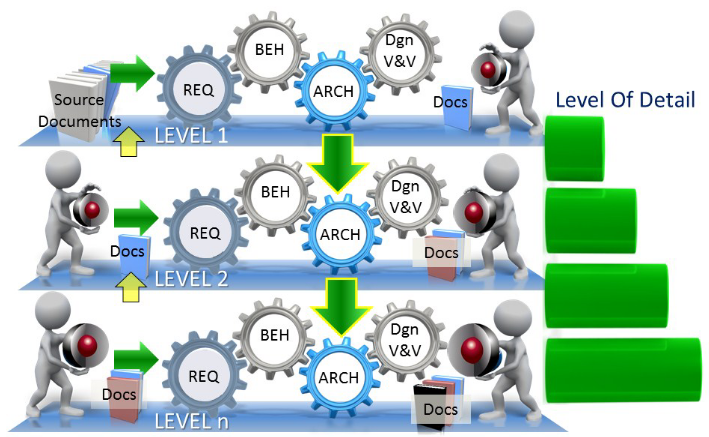
\includegraphics[keepaspectratio,width=.7\textwidth]{MBSE-ps.png}
  \caption[A Model-Based Systems Engineering process.]{A Model-Based
Systems Engineering process; REQ stands for requirements, BEH for
behavior, ARCH for architecture, Dgn V\&V for design verification and
validation. This figure is an excerpt from \cite{Long2011}.}
  \label{fig:MBSE-ps}
\end{figure}

In the case where the digital system being designed is a
safety-critical system, an MBSE process will often employ formal
models as the design formalism. Thus, these models enable a certain
extent of mathematical reasoning to prove that safety properties are
met during the design V\&V phase (cf. Figure~\ref{fig:MBSE-ps}).

To assist the engineers in the design and the implementation of
safety-critical digital systems, the CAMIN team came up with a process
called the ``\hilecop{} methodology'' \cite{Andreu2009}.  This
methodology follows the principles of a MBSE process and relies on
several transformations going from abstract models to concrete FPGA
(Field-Programmable Gate Array) or ASIC (Application-Specific
Integrated Circuit) implementations through the production of VHDL
code. Figure~\ref{fig:hilecop-wf} details the global workflow of
\hilecop{}.

\begin{figure}[H]
\centering
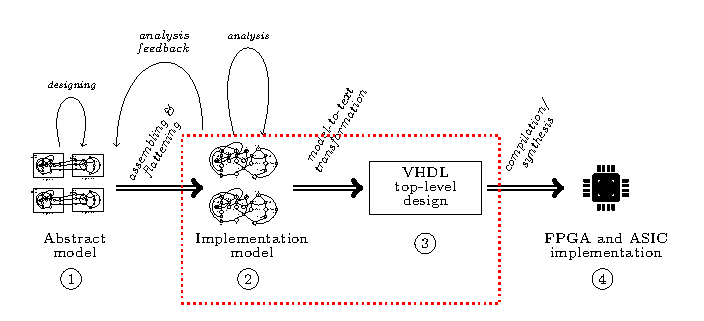
\includegraphics[keepaspectratio=true,width=\textwidth]{hilecop-wf.eps}
\caption[Workflow of the \hilecop{} methodology.]{Workflow of the
  \hilecop{} methodology; horizontal double arrows indicate the
  transformation phases, i.e. the refinement phases in MBSE terms;
  simple arrows indicate different kinds of operations performed at a
  given step.}
\label{fig:hilecop-wf}
\end{figure}

In Figure~\ref{fig:hilecop-wf}, Step~1 corresponds to the design phase
of a digital system. At this step, the user produces a model of the
required system; the leveraged model formalism is a graphical
formalism based on component diagrams and specific Petri nets (PNs).
In Figure~\ref{fig:hilecop-wf}, the transformation from Step~1 to
Step~2 flattens the model. The internal behaviors of separate
components are connected according to the interface compositions, and
embedding component structures are removed. The result of this
transformation step is a global PN that represents the internal
behavior of the digital system.  The class of PNs used in \hilecop{}
has been specifically devised for the design of safety-critical
digital systems; a first thesis has formalized the execution semantics
of these PN models \cite{Leroux2014}. What makes them a very
particular kind of models is their \textit{synchronous} execution
semantics. This semantics denotes from the standard
\textit{asynchronous} execution of PNs.  Due to its mathematical
foundations, a PN model can be analyzed, and a proof that a given
model meets some properties can be automatically produced through the
direct analysis of the structure or through the use of model-checking
techniques. This feature of PNs has been one of the reason of the
adoption of this formalism as \hilecop{}'s base formalism. A thesis
has been dedicated to the development of new methods to analyze the
\hilecop{} PN models \cite{Merzoug2018}. The analysis phase is here to
convince the engineers that they are indeed designing a safe
system. The analysis process is a round trip between Step~1 and
Step~2.  It aims at producing a model that is conflict-free (see
Section~\ref{sec:hilecop-models} for more details about the definition
of a conflict), bounded, and deadlock-free, using model-checking
techniques.  After several iterations, the model should reach
soundness and is then said to be \emph{implementation-ready}.

In Figure~\ref{fig:hilecop-wf}, from Step~2 to Step~3, \vhdl{} source
code is then generated by means of an automatic model-to-text
transformation. The generated code describes a \vhdl{} design, i.e. a
textual description of a hardware system, which has an interface
defining input and output ports and an internal behavior called an
architecture.

From Step~3 to Step~4, the \vhdl{} compilation/synthesis and the FPGA
programming, or ASIC realization, are finally performed using
industrial tools. At the end of Step~4, the designed circuit is
physically built on an FPGA device or an ASIC.  What happens between
Step~3 and Step~4 appears as a black box in the whole \hilecop{}
methodology. Therefore, we will not consider this transformation
phase, which will not be verified.

\subsection{Verifying the \hilecop{} methodology}
\label{sec:verif-hilecop}

The use of Petri nets as a base model is one of the major advantage of
the \hilecop{} methodology. All the analysis tools that accompany the
Petri net formalism, and allow us to prove that the models meet some
required properties, qualify the \hilecop{} methodology as a formal
method for the design and implementation of safety-critical digital
systems. However, the advantages provided by the use Petri nets would
be lost if one of the transformations performed during the process
changes the input model in a way that would alter its behavior. Thus,
the engineers would have specified a perfectly correct digital system
but would never obtain the expected circuit on a physical device. In
order to reinforce the confidence in the \hilecop{} methodology, the
goal of our work is to verify, by establishing a formal proof, that
the model-to-text transformation from Step~2 to Step~3 (i.e. the
framed part with red dotted lines in Figure~\ref{fig:hilecop-wf})
preserves the behavior of the input models into the generated \vhdl{}
designs. We choose to carry out this task as a deductive verification
task.  We aim at proving a theorem stating that the \hilecop{}
model-to-text transformation is \textit{semantic-preserving}. This
theorem will be of the following form: for all PN model, input to the
\hilecop{} transformation, the generated output \vhdl{} design behaves
similarly at execution time. Section~\ref{sec:proof} formally presents
our behavior preservation theorem, and thus, what we mean about the
similarity of execution between a PN model and a \vhdl{} design.

One could argue that to qualify the entire \hilecop{} methodology, one
has to verify all the transformations used in the methodology,
i.e. consider also the transformation from Step~1 to Step~2, and the
transformation from Step~3 to Step~4. However, we shall say that:

\begin{itemize}
\item The transformation from Step~1 to Step~2 changes the structure
  of the component-based input model. Even if the removal of the
  component structures induces some structural rearrangements, the
  behavior of the flattened model is almost similar to the one of the
  component-based model. Therefore, we argue that verifying that this
  transformation is semantic-preser\-ving is an easy enough task.

\item The transformation from Step~3 to Step~4 is performed by
  industrial tools. We rely on these tools because they are widely
  used in the industry for the development of safety-critical systems
  (e.g. cadence tools in aerospace and defense domains). Moreover, the
  compiler/synthesizer used at this stage of the methodology is a
  proprietary product. Thus, we don't have any access to the code of
  this program. % Moreover, the compiler/synthesizer performs a lot of
  % optimizations over the input \vhdl{} code. Even with a provided
  % access to the code, verifying such an optimizing compiler would not
  % possible within the time-span of this thesis.
\end{itemize}

% Now that we have clarified the nature of the verification task we want
% to achieve, we can state our research question as follows:

% \begin{center}
%   \textsc{Can we prove that the model-to-text transformation described
%     in the \hilecop{} methodology is semantic preserving?}
% \end{center}

\subsection{Related work}
\label{sec:related-work}

The verification task we want to achieve is really close to the formal
verification of compilers for programming languages. Compiler
verification has been widely explored, and many works are accessible
in the literature \cite{Dave2003}. The major source of inspiration of
this work has been the work done on the \ccert{} certified C compiler
\cite{Leroy2009}. Thus, we argue here that the scientific interest of
our research comes from the comparison between the methods used to
perform our verification task and the methods used to perform similar
verification task in other domains such as compiler verification. The
following research questions arises:

\begin{itemize}
\item What are the similarities and the differences between the
  \hilecop{} transformation and other transformation situations
  (compilers, model transformations\dots)?
\item Is there a strategy to perform the verification of the
  \hilecop{} transformation?
\item How far the correspondence holds between this strategy and the
  strategy used in other transformation situations such as compiler
  verification?
\end{itemize}

To achieve the formal verification of \hilecop{}, our approach is
similar to what has been done for the \ccert{} compiler. The idea is
to formalize the semantics of the source and target languages, and
verify that the transformation preserves the semantics of any input
model. In the thesis, we propose both to perform the formalization
work on ``paper'' and mechanize it within the \coq{} proof assistant
\cite{Bertot2004}.

In the case of \hilecop{}, some specificities of the source and target
languages introduce additional technical difficulties in the process
of formal verification. A first difference pertains to \hilecop{}'s
high-level formalism (the input language), which is quite
abstract. This formalism depends on PNs, and thus is not a common
programming language.

A second difference is about the \vhdl{} language (the output
language).  Similarly to the PN models used in \hilecop{}, the \vhdl{}
language is not a common programming language as its purpose is both
the structural and behavioral description of hardware
circuits. % Although previous work has been conducted toward the
% formalization of the \vhdl{} semantics \cite{Kloos2012}, a semantics
% that is able to both handle all the constructs in the generated
% programs, and facilitate the proof of behavior preservation, still
% needs to be designed.

\todo[inline]{ Here put the literature review.}

To further motivate the necessity of the verification task, the
development of neuroprostheses by the INRIA CAMIN team is at the base
of the creation of the Neurrinov
company\footnote{\url{http://neurinnov.com/}}. The Neurrinov company
is now looking towards the industrial development of such
neuroprostheses. We hope that once the verification performed on the
\hilecop{} methodology, it will help to obtain the CE certification,
related to the EU 2017/745 regulation text, necessary to qualify the
neuroprostheses as eligible for the medical market.

Moreover, the \hilecop{} methodology comes with a working
implementation based on the Eclipse framework . This software is
currently used by the engineers of the Neurinnov company to design the
digital systems having a part in safety-critical implantable medical
devices.

To the purpose of formal verification, we will implement the
\hilecop{} model-to-text transformation leveraging the functional
language of the \coq{} proof assistant. However, after the
mechanization of the proof of semantic preservation, we could use the
extraction feature of the \coq{} proof assistant to produce the
implemented transformation as an \ocaml{} program. Then, we will be
able to connect this program to the existing \hilecop{} software in
order
to use the verified version of the transformation.\\

This article is structured as
follows. Section~\ref{sec:hilecop-models} presents the specific kind
of Petri net models which are the input models of \hilecop{}'s
model-to-text transformation.  Section~\ref{sec:hvhdl} gives a formal
definition of the syntax and semantics of a subset of the \vhdl{}
language that we call \hvhdl{}. \hvhdl{} is the target language of the
programs generated by \hilecop{}'s model-to-text transformation?
Section~\ref{sec:m2t} presents the algorithm of the transformation and
its implementation with the \coq{} proof assistant.
Section~\ref{sec:proof} details the semantic preservation theorem
expressing that the \hilecop{} transformation is semantic-preserving.
It also gives the high-level theorems and lemmas involved in the proof
of the semantic preservation theorem.  Finally,
Section~\ref{sec:concl} ends the article, and outlines the
perspectives regarding the full completion of the task of proving that
the \hilecop{} transformation is semantic-preserving.

\section{Models of digital systems in \hilecop{}}
\label{sec:hilecop-models}

\section{A target language: \hvhdl{}}
\label{sec:hvhdl}

\section{Model-to-text transformation}
\label{sec:m2t}

\section{Proof of semantic preservation}
\label{sec:proof}

\section{Conclusion}
\label{sec:concl}


\bibliography{references}

\end{document}
